%!TEX root = ../document.tex

During our interviews, we briefly observed Christof Dorner from Readmill during his work. He showed us how he develops a feature: He choose a task from the bug and feature tracker Trello, created a git branch locally, fixed the problem, wrote tests for it and eventually opened a Pull Request on Github with the finished code to have it code reviewed and deployed. Here we gained the insight, that a friction-less and uninterrupted flow is important. This can be achieved by customizing and constantly improving the used tools. Christof mentioned how he improved the flow over time, e.g. making tests run instantly on each change or working with a decentralized source code management tool.

We also observed the two current Bachelor projects from the HPI EPIC chair. Both bachelor projects work with real customer data as well as existing legacy code. During observation we noticed that one problem they face is a disconnect between understanding the code in the editor and the data in the database. This lead to switching back and forth between the code editor and the HANA database studio as well as guessing values for variables in the queries.

Additionally to the interviews and observations, we took our own experience of developing applications with databases into account as well as incorperated experiences from the seminar \emph{Enterprise Application Programming Model Research 2012} at the HPI EPIC chair~\footnote{\url{https://github.com/lauritzthamsen/infrarecord/}}.

\begin{figure}
    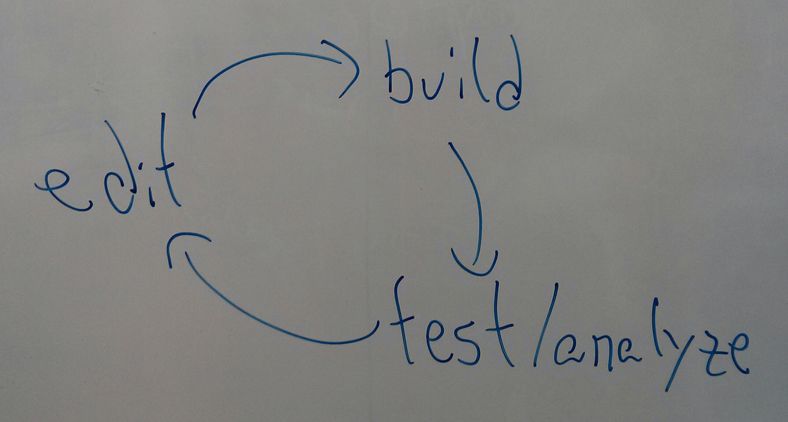
\includegraphics[width=\linewidth]{images/EditBuildTest.jpg}
    \caption{The code development cycle drawn on a whiteboard during the project week}
    \label{fig:cycle}
\end{figure}

While investigating common workflows of software developers, we realized that they often follow the cycle depicted in Figure~\ref{fig:cycle}. Before entiring that cycle, the software developer chooses the scope of the feature and does all the necessary work to have an actionable coding task at hand. When the actual code generation begins, the developer starts the cycle by editing code. Depending on the programming language, the code has to be built or otherwise brought into a testable state. Then the code changes are tested, for example by running unit tests or by running and manually testing the application. This cycle repeats, until the developer is satisfied with the results.

Once this cycle became apparent to us, we investigated the components the cycle operates on. Especially from the experiences of the bachelor projects we realized that in the editing step, the develoepr has no access to the data context that the code will eventually be executed in the test/analyze step. There is a disconnect between the editor and the application runtime. The developer writes down their thoughts as code in the edit step and later on the program is eventually interpreted by the machine. This is also the reason why the cycle exists in the first place, because developers have to continously test the assumptions they made about the behaviour of their program. We realized that in the cycle every execution of the cycle is an interruption to the developer. Thus it would be better if the cycle would not exist in the first place, or if at least it could be so small that it becomes unnoticable to the developer. One important requirement for this is that already during writing code, the developer has access to the context the program will be executed in later. When working with an external data source, the actual data become this important context.

From this we gained our third insight, that also became the leading insight for the rest of the project:

\begin{quote}
\emph{Code needs data context}
\end{quote}